\section{Results}
\label{sec:results}

\begin{figure}[t]
\centering
\includegraphics[width=\columnwidth]{fig_transfer_heatmap.pdf}
\caption{Cross-generator $8{\times}8$ transfer matrix (binary F1, gen-1 vs.\ gen-2+). Mean cross-generator F1\,=\,0.810 [95\% CI: 0.796, 0.822]; uniformly high off-diagonal values confirm depth signal transfers across five families without calibration.}
\label{fig:transfer-heatmap}
\end{figure}

\subsection{Depth Classification Performance}
\label{sec:results-classification}

\looseness=-1 The 7-feature ensemble achieves 3-class LOGO F1\,=\,0.762 (95\% CI [0.758, 0.766]; $N$\,=\,37{,}058) across eight generators from five families (Table~\ref{tab:logo-results}); cross-generator F1 spread of 9.1\,pp captures generator selection uncertainty.
This 3-class metric is inflated by shared gen-0 seeds (per-class gen-0 F1\,$\approx$\,0.94; \S\ref{sec:generation}); we therefore report \textbf{leak-free binary F1} (gen-1 vs.\ gen-2+)\,=\,0.694 (CI [0.688, 0.700]) throughout, excluding gen-0 entirely.
Per-generator binary F1 ranges from 0.633 (Mistral-7B) to 0.724 (Pythia-2.8B; std.\ dev.\ 0.028), with the primary difficulty at the gen-1\,/\,gen-2+ boundary (Appendix~\ref{app:confusion}).

\paragraph{Cross-model generalization.}
\looseness=-1 Cross-model chains (randomly selected generator per step) yield binary F1\,=\,0.830 (95\% CI [.818, .841]; Appendix~\ref{app:cross-model-detail}) under 5-generator LOGO.\footnote{Pythia-2.8B/1B, OLMo-2-1B, Qwen3-0.6B/1.7B; generator-level LOGO with bootstrap CIs ($n$\,=\,1{,}000).}
Single-generator transfer confirms the signal is not a mixed-chain artifact (mean transfer F1\,=\,0.810; Figure~\ref{fig:transfer-heatmap}; full $8{\times}8$ matrix: Appendix~\ref{app:transfer}; LOFO\,=\,0.686).
ANOVA confirms generator identity contributes ${<}1$\% of feature variance ($\eta^2_{\text{gen}} \leq 0.009$; Appendix~\ref{app:cross-model-detail}).
A scale effect emerges: smaller models achieve higher F1 (Pythia-2.8B: 0.724 vs.\ Mistral-7B: 0.633), partly due to same-family affinity with the Pythia-410M reference (spread $\leq$0.013; \S\ref{sec:results-differential}).
An end-to-end QLoRA classifier reaches 3-class F1\,=\,0.905 (within-model 5-fold CV; $+$10.0\,pp; Appendix~\ref{app:qlora}), evidence that additional depth signal resides in token-level representations. On instruct data, QLoRA recovers to 0.89--0.91 (within-model; Appendix~\ref{app:instruct}).

\paragraph{Confound controls.}
\looseness=-1 Length-matched subsampling yields binary F1\,=\,0.724 (vs.\ 0.770; Appendix~\ref{app:length}); independent-seed evaluation with disjoint pools (F1\,=\,0.680; Appendix~\ref{app:seed-control}), so the classifier captures generative degradation rather than seed-specific content.

\paragraph{Error analysis.}
\looseness=-1 The gen-1\,/\,gen-2+ boundary is the primary failure point: depth-2 samples (the shallowest within the 2+ class) exhibit the highest error rate (48.4\%), decreasing monotonically to 20.3\% at depth-4 (Appendix~\ref{app:error-analysis}) due to insufficient accumulated drift beyond the large gen-0$\to$gen-1 distributional shift.
Error rates decrease monotonically at deeper generations ($\leq$29.2\% at gen-3+); DDR signal thus strengthens with chain length.

\begin{table}[t]
\centering
\footnotesize
\caption{8-generator LOGO macro-F1 (bootstrap 95\% CIs, $n$\,=\,1{,}000). Binary F1 excludes gen-0. $^{\dagger}$3-class F1 has upward bias from shared gen-0 seeds; independent-seed controls confirm the signal (F1\,=\,0.680; Appendix~\ref{app:seed-control}).}
\label{tab:logo-results}
\resizebox{\columnwidth}{!}{%
\begin{tabular}{@{}llcccc@{}}
\toprule
\textbf{Model} & \textbf{Family} & \textbf{Params} & \textbf{Bin F1} & \textbf{95\% CI} & \textbf{3-class F1}$^{\dagger}$ \\
\midrule
Pythia-2.8B     & Pythia  & 2.8B & \textbf{0.724} & [.707, .742] & 0.798 \\
Pythia-1B       & Pythia  & 1.0B & 0.718 & [.700, .735] & \textbf{0.806} \\
Qwen3-1.7B     & Qwen    & 1.7B & 0.709 & [.693, .726] & 0.772 \\
Llama-3.2-3B   & Llama   & 3.2B & 0.697 & [.680, .713] & 0.775 \\
OLMo-2-1B      & OLMo    & 1.5B & 0.695 & [.679, .711] & 0.781 \\
Qwen3-8B       & Qwen    & 8.2B & 0.692 & [.674, .708] & 0.714 \\
Qwen3-0.6B     & Qwen    & 0.6B & 0.691 & [.673, .709] & 0.780 \\
Mistral-7B     & Mistral & 7.0B & 0.633 & [.617, .648] & 0.682 \\
\midrule
\multicolumn{3}{l}{\textbf{Average (8-gen LOGO)}} & \textbf{0.694} & [.688, .700] & \textbf{0.762} \\
\multicolumn{3}{l}{\textbf{LOFO (family-level)}} & 0.686 & --- & --- \\
\bottomrule
\end{tabular}}
\end{table}

\subsection{Differential Depth Response}
\label{sec:results-differential}

\paragraph{Formal definition.}
\looseness=-1 For feature $f$ measured across depths $d \in \{0,1,2{+}\}$, we define its \emph{depth sensitivity} as $\text{DDR}(f) = |\rho(\text{depth}, f)|$, where $\rho$ is Spearman correlation over all per-text measurements.
A feature is classified as \emph{drifting} if Cohen's $d > 0.50$ between adjacent depths, or \emph{stationary} if $d < 0.15$; the two-cluster structure is robust across $\varepsilon \in [0.10, 0.75]$ ($k$-means silhouette\,=\,0.660, $p{=}0.030$; exhaustive split enumeration ranks this partition first; independent replication in all eight generators; Appendix~\ref{app:ddr-validation}).
\looseness=-1 Recursive inputs grow increasingly self-typical~\citep{markovian_chains}; this predicts location drift with shape invariance (confirmed across nucleus, greedy, and top-$k$ strategies; Appendix~\ref{app:decoding-strategy}).

\looseness=-1 Figure~\ref{fig:ddr-trajectory} reveals the dichotomy: central-tendency features (entropy mean, TTR, hapax ratio) decline monotonically with depth, while shape features (entropy max, tail decay, entropy min) remain flat (per-feature distributions: Appendix~\ref{app:feature-distributions}; qualitative chain example: Appendix~\ref{app:qualitative}).
The partition is binary ($k{=}2$; silhouette\,=\,0.660), with entropy std as the sole \emph{intermediate} member ($d{=}0.46$, $|\rho|{=}0.16$), distinct from three near-stationary features ($d < 0.10$; Appendix~\ref{app:ddr-validation}).

\begin{figure}[t]
\centering
\includegraphics[width=\columnwidth]{fig1_differential_response.pdf}
\caption{Differential depth response (DDR). Drifting features (red; $|\rho| > 0.60$, effect size $d{=}0.74$--$1.05$) shift monotonically with generation depth; near-stationary features (blue; $d \leq 0.10$) are approximately preserved; entropy std (purple; $d{=}0.46$) is intermediate. Diamonds: cross-generator means; dots: per-generator values.}
\label{fig:feature-drift}
\end{figure}

\looseness=-1 Pooled Spearman correlations corroborate the split: drifting features show $|\rho| > 0.60$ (hapax ratio $-0.64$, TTR $-0.62$, entropy mean $-0.60$) vs.\ $|\rho| \leq 0.16$ for entropy max and tail decay; entropy min reaches $|\rho|{=}0.40$ due to its gen-0/gen-1 boundary sensitivity (discussed below). This persistent magnitude gap defines the DDR partition (Figure~\ref{fig:feature-drift}).

\begin{figure}[t]
\centering
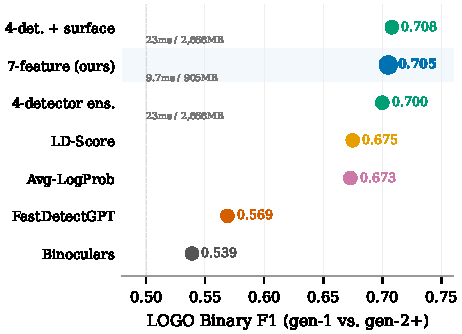
\includegraphics[width=\columnwidth]{fig3_baseline_comparison.pdf}
\caption{LOGO binary F1 vs.\ inference cost (8-gen pooled). The 7-feature ensemble (one 410M model) matches multi-detector ensembles (1.4B total) at ${\sim}2.4\times$ lower cost. RTX 5090 timings.}
\label{fig:baseline-ci}
\end{figure}

\paragraph{Quantification.}
\looseness=-1 Cohen's $d$ shows a ${\geq}8{\times}$ gap between drifting ($d{=}0.74$--$1.05$) and near-stationary ($d < 0.10$); KS, Glass's $\Delta$, Cliff's $\delta$ corroborate (Appendix~\ref{app:ddr-validation}).
Entropy min and tail decay are \emph{boundary features}: entropy min is near-stationary for gen-1/gen-2+ ($d{=}0.016$) but sensitive at gen-0/gen-1; tail decay passes two one-sided tests (TOST) equivalence (Appendix~\ref{app:tost}) for only 4/8 generators (per-generator $|d|{=}0.07$--$0.22$).
\paragraph{Validation.}
\looseness=-1 Each hold-out generator independently recovers the identical partition (silhouette 0.505--0.760); TOST confirms near-stationarity for entropy min (8/8) and entropy max (6/8); permutation testing confirms the split as non-random ($p{=}0.030$). Per-feature convergence dynamics (Figure~\ref{fig:convergence}), per-family DDR consistency (Appendix~\ref{app:family-ddr}), and causal feature analysis (Appendix~\ref{app:ddr-causality}) appear in Appendices~\ref{app:ddr-validation}--\ref{app:convergence}.

\paragraph{Feature complementarity.}
\looseness=-1 The full 7-feature set (F1\,=\,0.771, 10-fold stratified cross-validation) outperforms surface-only (0.688) and reference-only (0.713; McNemar $p \approx 0$; Appendix~\ref{app:ablation-table}).
Group ablation (10-fold stratified CV) confirms complementarity: 3-class F1 gains $+$5.3\,pp when non-drifting features are added (drifting-only 0.716, all-7 0.769), while binary detection is already saturated by location drift alone (drifting-only 0.697 vs.\ all-7 0.700); shape stability thus contributes to depth \emph{grading}, not detection.
TTR and hapax ratio ($r = 0.97$) are retained for marginal LOFO gains (Appendix~\ref{app:lofo}).

\paragraph{Cross-family reference models.}
\looseness=-1 Alternative references (OLMo-2-1B, Qwen3-0.6B) yield F1 spread of only 0.013 (Appendix~\ref{app:cross-ref}); same-family proximity may inflate Pythia F1 by up to 1.2\,pp, but the DDR partition is preserved.

\paragraph{Temperature and prompt-type sensitivity.}
\looseness=-1 All four tested generators degrade at $t{=}0.9$ ($-$9.3 to $-$26.0\,pp binary F1; Appendix~\ref{app:sampling-sensitivity}); continuation chains show the strongest drift (F1\,=\,0.781; Appendix~\ref{app:prompt-type}).
The DDR partition hierarchy is preserved across temperatures (Appendix~\ref{app:ddr-temp-stability}), including cross-temperature transfer (Appendix~\ref{app:cross-temp}); random word replacement at 10\% degrades binary F1 by only 8\,pp (Appendix~\ref{app:human-edit}).


\subsection{Comparison with Detection Baselines}
\label{sec:results-baselines}

\begin{table}[t]
\centering
\footnotesize
\caption{Depth classification (8-gen LOGO, pooled). Binary F1 excludes gen-0. 7-feature: one 410M model; 4-det ensembles: two models, 1.4B. QLoRA (\S\ref{sec:results-classification}) uses full token sequences (within-model 5-fold CV, not LOGO), serving as an information-asymmetric ceiling.}
\label{tab:baselines}
\resizebox{\columnwidth}{!}{%
\begin{tabular}{lcccc}
\toprule
\textbf{Method} & \textbf{Feat.} & \textbf{3-class F1} & \textbf{Bin F1} & \textbf{ms/text} \\
\midrule
4-det.\ + surface     & 6 & \textbf{0.795} & \textbf{0.708} & 22.8 \\
4-detector ens.\      & 4 & 0.785 & 0.700 & 22.8 \\
7-feature (ours)      & 7 & 0.774 & 0.705 & \textbf{9.7} \\
\midrule
Avg-LogProb           & 1 & 0.707 & 0.673 & --- \\
FastDetectGPT         & 1 & 0.660 & 0.569 & --- \\
LD-Score              & 1 & 0.630 & 0.675 & --- \\
Binoculars            & 1 & 0.411 & 0.539 & --- \\
\bottomrule
\end{tabular}}
\end{table}

\looseness=-1 We next ask whether existing detection methods, designed for binary real-vs-synthetic classification, incidentally capture depth structure, repurposing four detection scores as ordinal depth predictors under identical XGBoost and LOGO conditions (Table~\ref{tab:baselines}).
The strongest baseline is a 4-detector + surface feature ensemble (binary F1\,=\,0.708), which pools four detection scores with TTR and hapax ratio; among individual detectors, Avg-LogProb provides the most meaningful single-feature comparison.

\looseness=-1 The 7-feature ensemble matches the 4-detector+surface ensemble on binary F1 (0.705 vs.\ 0.708; Figure~\ref{fig:baseline-ci}) at ${\sim}2.4\times$ lower cost, though the latter leads by 2.1\,pp on 3-class F1 (0.795 vs.\ 0.774); both surpass individual detectors by 3.0--16.6\,pp.
The DDR decomposition explains why depth discrimination is achievable: location features carry the signal and shape features enable cross-generator transfer (\S\ref{sec:discussion}), all with a single 410M reference model; ordinal-specific methods (CORAL, Frank-Hall) yield comparable F1 (Appendix~\ref{app:classifier}).
Among individual detectors, LD-Score and Avg-LogProb best capture depth structure (binary F1\,=\,0.675 and 0.673); FastDetectGPT captures 3-class ordering (F1\,=\,0.660) but struggles with binary depth separation (F1\,=\,0.569); Binoculars is least informative (binary F1\,=\,0.539).
Concurrent iterative-generation studies use different chain operators and cannot be directly included as depth baselines (Appendix~\ref{app:iterative-comparison}).

\begin{figure*}[t]
\centering
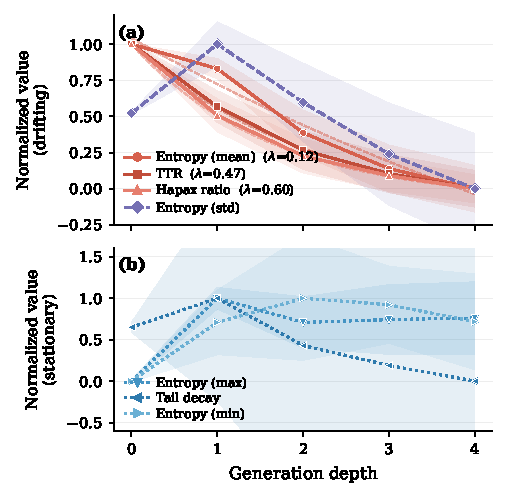
\includegraphics[width=\textwidth]{fig_convergence_dynamics.pdf}
\caption{Feature convergence dynamics. (a)~Drifting features (red) and intermediate entropy std (purple): $|d| > 0.46$ by gen-2+. (b)~Near-stationary features (blue): $|d| < 0.25$ at all depths. Shape stability persists across chain lengths.}
\label{fig:convergence}
\end{figure*}
